\documentclass[10pt,conference]{IEEEtran}
%\documentclass[a4paper,12pt]{article}

\usepackage{cite,latexsym,times,epsf,amsmath,amssymb,amsfonts,graphicx}
\usepackage{epstopdf}
\usepackage{graphicx}
\usepackage{subfigure}
\usepackage{multirow}
\usepackage{algorithmic}
\usepackage{algorithm}
\usepackage{verbatim}
\renewcommand{\algorithmicrequire}{\textbf{Input:}}
\renewcommand{\algorithmicensure}{\textbf{Output:}}
\renewcommand{\baselinestretch}{0.95}
\renewcommand{\algorithmicforall}{\textbf{Foreach}}
\renewcommand{\algorithmicendfor}{\textbf{}}

\begin{document}
\title{WhiteMesh: Leveraging White Spaces in Multihop Wireless Topologies}
\author{TBA \\
Dinesh Rajan, and Joseph Camp\\ 
%Department of Electrical Engineering,\\ Southern Methodist University (SMU), Dallas, TX \\
%\{camp\}@smu.edu  \\
}


%\documentclass[10pt]{article}

%\usepackage{xkvltxp}


\maketitle


\begin{abstract}

Wireless mesh networks were previously thought to be an ideal solution for
large-scale Internet connectivity in metropolitan areas.  However, in-field
trials revealed that the node spacing required for WiFi propagation 
induced a prohibitive cost model for network carriers to deploy. The digitization 
of TV channels and new FCC regulations have reapportioned spectrum for data 
networks with far greater range than WiFi due to lower carrier frequencies. 
Also, channel occupancy of change the performance of wireless network across 
both ISM bands and white space bands. In this work, we consider how these white 
space bands can be leveraged in large-scale wireless mesh network deployments 
with in-field measured channel capacity. In particular, we present an integer 
linear programming model to leverage diverse propagation characteristics and 
the  channel occupancy of white space and WiFi bands to deploy optimal WhiteMesh 
networks. Since such problem is known to be NP-hard, we design a measurement driven 
heuristic algorithm, Band-based Path Selection (BPS), which we show approaches 
the performance of the optimal solution with reduced complexity.  We additionally 
compare the performance of BPS against two well-known multi-channel, multi-radio 
deployment algorithms across a range of scenarios spanning those typical for 
rural areas to urban areas. In doing so, we achieve up to 160\% traffic achieved 
gateways gain of these existing multi-channel, multi-radio algorithms, which are 
agnostic to diverse propagation characteristics across bands.  Moreover, we show 
that, with similar channel resources and bandwidth, the joint use of WiFi and 
white space bands can achieve a served user demand of 170\% that of mesh networks 
with only WiFi bands or white space bands, respectively. Further, through the 
result, we leverage the channel occupancy and spacing impacts on white mesh
network and study the general rules of band selection.



\end{abstract}

%
% Introduce the background and problem, calim contribution

\section{Introduction}
\label{sec:introduction}

% Background multiband networks, hetergeneous networks, vehicular applications
% Introduction of white spcae.
% Process:
% Clearify the channel in different cities
% Introduce 2 possible gain: 1. reduce # mesh nodes 2. given topology get average capacity 
FCC adopted rules to allow unlicensed radio transmitters to operate in the white space freed from TV band since 2010~\cite{fccwhitespace}. White space is popularly referred to unused portions of the UHF and VHF spactrum includes, but not limited to 54M-72MHz,76M-88MHz,174M-216MHz,470M-608MHz,and 614M-806MHz ~\cite{whitespacewiki}.
To use these band, FCC ruling requires white space devices(WSDs) to learn of spectrum availability at their respective locations from a database of incumbents. For example, in Dallas/Fort Worth, TX, 482M-488MHz band should be yielded for TV channels, in Chicago, IL 470M-482MHz band is reserved for TV channels. ~\cite{broadband}
 These bands provides superior propagation and building penetration compared to licensed ISM Wifi bands like the 2.4 and 5GHz bands, holding rich poetntial for expanding broadband capacity and improving access for wireless users.

% Wireless mesh networks
Wireless mesh network is able to provide broadband Internet access to large contiguous areas through less mesh nodes equipped with WSD due to the propagation characteristic of ISM bands. White space mesh is an economic way to provide backhaul internet service in rural area or other low density area employing the propagation characteristics.
White space could also be used to improve the urban or high density area connectivity through lower interference channels. 

Mesh deployment requires selecting the number and locations to place mesh nodes to cover the whole area and the nodes are inter-connected in order to access to Internet gateway points.
Unfortunately, prior white space mesh placement research fails to address the compatibility of current existing devices, for instance, iPhone, Mac Laptop do not have white space radios to access white space gateway points. For a realistic mesh network, the end hop to the client need to be able to work in ISM Wifi band. 
To appreciate the multiband mesh deployment problem, it is important to understand the differences between white spaces and the popular ISM bands where Wifi devices operate. First, in FCC rules, users in white space band have to yield primary users.Before enter a white space channel, users have to detect the channel occupation. Second, white space band may suffer some unknown interference such as wireless Mic. Such devices may turn on at anytime without warning. Third, white space is cleaner than ISM bands since most of the TV stations have stopped using the bands. And also since in white space is in lower band, the coverage of these band is larger than higher frequency ISM band which could help to reduce the mesh nodes. According to these advantages and disadvantages, the balance between white space bands and ISM bands is possible to provide imporvement of mesh network. 

% AP location estimate 

% Paper focusing
This work focus on minimize the mesh nodes when gurantee the coverage and connectivity of the network.
We present FIXME mesh node placement algorithms so as to minimize the deployed nodes, guarantee the coverage, and mesh node inter-connectivity.


% 

% Contribution
% problem/environment propose
% algorithms
% 
The main contributions of our work are as follows:
\begin{itemize}
\item We formulate the hetergeneous mesh node placement problem as a FIXME problem.  

\item We propose a methodology to leverage the infulence of white space in mesh networks.

\item We propose FIXME algorithms to minimize the numberof deployed mesh nodes.
% Also should we consider the cost of different kind of nodes (1 radio, 2 radios, 3 radios )

\item We perform extensive outdoor experiments from multiple environments and simulations to evaluate the proposed algorithms.


\end{itemize}



%The remainder of this paper is organized as follows. In Section II, we present the multiband adaptation problem and proposed algorithms. Section III discusses experimental evaluation of the multiband algorithms. We conclude in Section IV.


% Multiband architecture and interference model Linear optimization model
\section{Multiband Mesh Architecture and Model}
\label{sec:architecture}

% Organization of the Sec
In this section, we first introduce the 
~\emph{Multiband Mesh Network Architecture}
with white space band propagation, connectivity and interference characteristics.
Then we analysis the architecture and formulate the architecture into a graph model with hypothesis.

\subsection{Multiband Mesh Network Architecture}
\label{subsec:architecture}
Generally ~\emph{Wireless Mesh Network} is been described as two-tiers:
Consisting of an access layer for clients to mesh nodes, and a backhual layer for interconnection from mesh nodes to gateway nodes with wired Internet connection ~\cite{akyildiz2005wireless}. 
Nodes in backhual layer are static.
Our work focus on ~\emph{Wireless Mesh Network} with ~\emph{White Space Frequency} in backhual layer. 
The clients devices in industrial, scientific and medical (ISM) band, such as iPhone, laptops, access to mesh node with independent channel of ISM band from backhual layer. 

% Explain multiband vs multichannel
A lot of efforts have been put on ~\emph{Multichannel Multi-radio Mesh Network} architecture focusing on ~\emph{Gateway Placement, Channel Assignment, Multihop Routing} problems ~\cite{si2010overview}.
~\emph{Multichannel} is a word mention different frequency channels with small gap, for instance the orthogonal WLAN channels in 2.4GHz from 2.412GHz to 2.484GHz with 22MHz gap.
We refer ~\emph{Multiband} with a combination of different frequency of large gap, such as a set 2.4GHz and 900MHz whose propagation characteristics are different.

% Explain propagation, factors of the environment and so on
Wireless propagation is the behavior of the signal loss characteristics when they are transmitting from one point to another.
The factors rule radio propagation are complex and diverse, and in most propagation models there are three basic propagation mechanisms: reflection, diffraction, and scattering ~\cite{andersen1995propagation}.
Wireless propagation could be affected by the daily changes of environment, weather, and atmosphere changes due to cosmos activities. 
In multiband mesh backhual layer, the nodes are usually installed on the top of buildings or towers. That makes a line of sight propagation model is a reasonable hypotheses for multiband mesh.
% propagation fomular, explain the band influence
In a popular propagation model \emph{Friis Model}, the received signal power of a node is represented as: 
\begin{equation}
\label{eq:friis}
P_r=P_t+G_t+G_r+20log_{10}(\frac{\lambda}{4\pi R})
\end{equation}

Path-loss exponent \emph{$\alpha$} is used to describe the environment factors, typically in outdoor environments range from 2 to 5.\cite{camp2006measurement}. 
The received signal could be different only related to the wavelength $\lambda$ represents band. 
The propagation difference makes the performance of radios in different bands vary with the same configuration in the same location. With the same received signal threshold, lower frequency band could have a larger propagation range $R$.

In multiband scenario, both wired ~\emph{Gateway Nodes} and ~\emph{Mesh Nodes} are equipped with multiple radios working in different frequency band, including ISM bands and white space bands. The radios could work simultaneously bringing more capacity to the network which is a evolution of ~\emph{Multi-channel Multi-Radio Mesh Network} with radios working in the same band in different channels.

\begin{figure}                                                                                                                     
%\vspace{-0.0in}
\centering
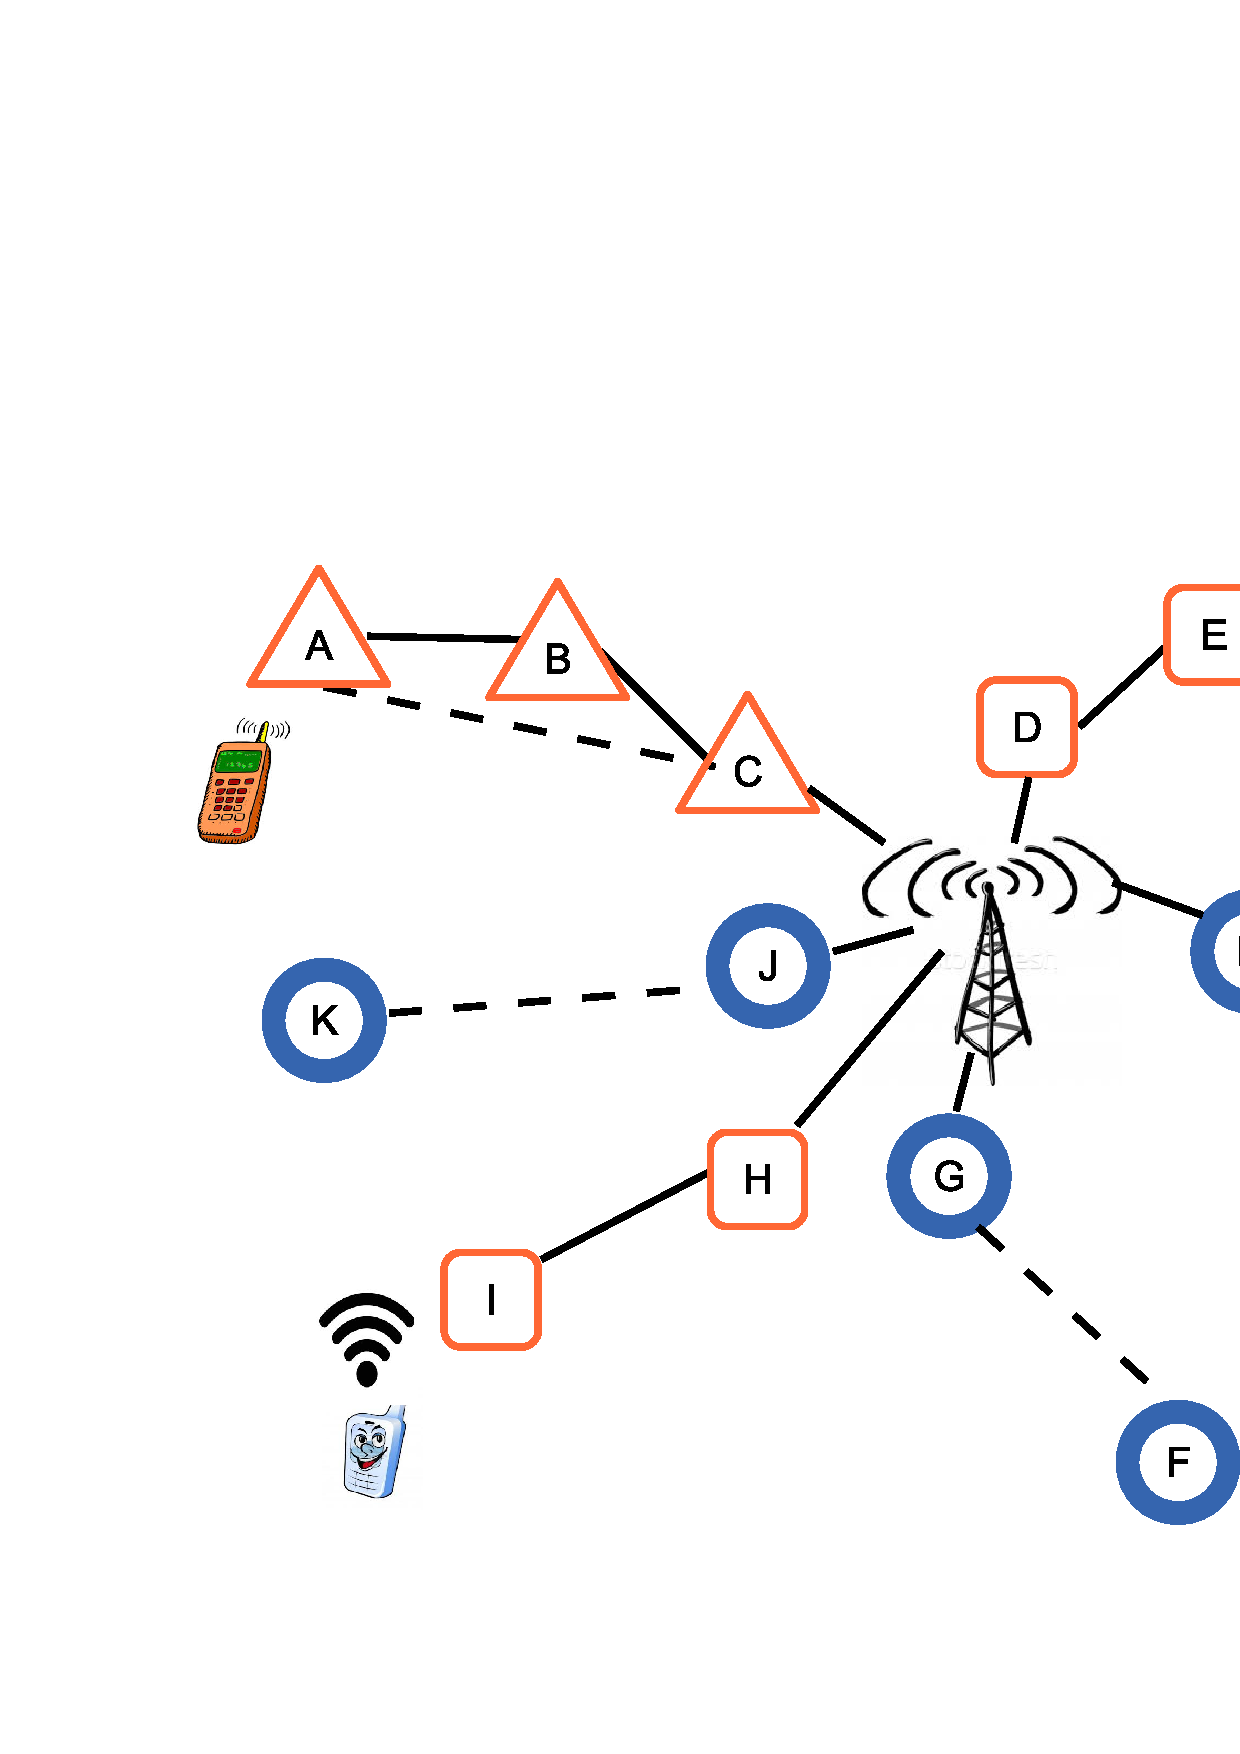
\includegraphics[width=74mm]{figures/interferencerange}
\vspace{-0.1in}
\caption{Multiband Communication and Interference Range}
\label{fig:interferencerange}
%\vspace{-0.0in}
\end{figure}


% Make multiband networks interesting 
The broadcast nature of the wireless medium makes it generate multiple access interference.
Employing ~\emph{White Space Band} in lower frequency brings advantages for mesh network, 1) more orthogonal bandwidth make the contention in the network lower,
 2) the propagation difference brings flexible topology by reduce connection hop counts in the network.
However, at the same time, ~\emph{White Space Band} also increase the interference range in the network making more interference in the same band. Both goods and bad are embedded in ~\emph{White Space Band} for mesh network.
In \ref{fig:interferencerange}, node ~\emph{N1} could connect to node ~\emph{N3} relay on node ~\emph{N2} in higher frequency band or through lower frequency band directly.
If under higher frequency band, link between node ~\emph{N4} and node ~\emph{N5} could reuse the higher frequency because they are out of the interference range of this high frequency band; however, if \emph{N1} and ~\emph{N3} use lower frequency band with less hop count, then ~\emph{N4} and ~\emph{N5} could not reuse the lower frequency due to the larger interference range.
To balance the larger communication range and larger interference range of white space band is a key issue in ~\emph{Multiband Mesh Network Channel Assignment}.

\subsection{Model and Problem Formulation}
\label{subsec:problem}

% Assumptions of the network
~\emph{Channel Assignment} is to assign radios between nodes in mesh network creating virtual links for network communication with minimum interference.
We consider a wireless mesh network formed by a set of stationary mesh nodes and wired gateway nodes. Each node is equipped with one or more radios in different bands. To clarify the ~\emph{White Space Band} influence, we assume radios in a node works in unique non-overlapping channels of multiple band, radios in two nodes share a common channel in the same band.
All the radios work under the same transmitting power, antenna with the same gains.
To model the connectivity, we adopt classical ~\emph{Protocol Model} from Gupta ~\cite{gupta2000capacity}. If the received signal is above the threshold, the link would have a communication capacity, otherwise, the link could not exist.
For the interference, when the received signal is above the interference threshold, there will be contention exist; otherwise, the signal will not influence other links.

The ~\emph{Gateway Nodes} and ~\emph{Mesh Nodes} locations have been known as input. In a network, ~\emph{Channel Assignment} naturally binds with a routing protocol for application, but have different target. We bind our model with a ~\emph{Shortest Path Routing} protocol for ~\emph{Channel Assignment} application and evaluation.

From the input nodes location, transmitting power, antenna gains, communication and interference threshold, and bind with ~\emph{Friis Model}, we can get ~\emph{Communication Range} and ~\emph{Interference Range} of each node in different band. 
We model the connectivity between mesh nodes by an undirected graph ~\emph{Connectivity Graph}, $C=(V,L,B)$, $V$ denotes the set of nodes, $L$ denotes the set of links, $B$ denotes the set of frequency bands. A pair of nodes have a link with capacity $C_l$ in $L$ of band $b$ in $B$, if they are physically located within each others communication range of a band. 

This model associates an interference range which is larger than the communication range for each node, defining the range up to which a transmitter can interference with the reception of a link. We extend the ~\emph{Conflict Graph} from Jain's work with a flexible approach for interference, $CG=(L_{i,j},I_{Set},B)$. $L_{i,j}$ is the active link, $I_{Set}$ includes all the links are physically inside the interference range, 

Our model is similar to ~\emph{Multichannel Model} in previous works ~\cite{tang2005interference,yuan2006cross,si2010overview}. However, in ~\emph{Multichannel Model}, the ~\emph{Communication Range} and ~\emph{Interference Range} in different channels are the same. The ~\emph{Multichannel Model} is unnecessary to consider the variation of range due to band propagation.
~\emph{Multiband Channel Assignment} work toward the same target as ~\emph{Multichannel Channel Assignment} to provide richer connectivity with minimum interference with the influence on topology from the new multiband factor.

The difficulty of the problem is that we can not know the interference before we assign channel to each node. Previous works have proposed ~\emph{Coloring, Cluster, Independent Set, Mixed Linear Integer} methodology to approach the solution of ~\emph{Multichannel Channel Assignment} ~\cite{mishra2005weighted,peng2012efficient,tang2005interference}. 
However, they fails to distinguish the ~\emph{Multi-hop} and ~\emph{Conflict Graph} variation among multiple bands.
To approach the optimization channel assignment, we develop a mixed linear integer model to fit the multiband scenario. We also analyze the intra-relation between the ~\emph{Hop Counts} and ~\emph{Conflict Graph} and propose a partition and a heuristic approaching for this problem.

\subsection{Evaluation Metric}
\label{subsec:metric}
~\emph{Mesh Network} is designed to provide service for clients. The goal of a backhual network is to maximize its overall goodput within a unit time. 
This enables the network to support more end-user flows, and in turn more number of users. To evaluate the assignment, we use the idea of ~\emph{Gateway Goodput} of the network. The gateway goodput X of a network is defined as

\begin{equation}
\label{eq:goodput}
X=\sum_{g \in G, v \in V}C(g,v)
\end{equation}

In ~\cite{robinson2008adding}, Robinson proves the bottle neck of mesh network capacity is the gateway wireless connection. The gateway goodput is the traffic arrive at the gateway node and relay to the wired Internet. The goodput performance is correlated with gateway placement, channel assignment and routing. Our work focus on the channel assignment after gateway placement done, binding with shortest path routing. Jointly optimize the problem is out of the paper topic.


% Mixed Linear Optimization
\subsection{Mixed Integer Linear Programming Formulation}
\label{subsec:linearopt}

We now present a mixed integer, linear programming formulation for 
optimizing gateway goodput when selecting channels
for WhiteMesh topologies across diverse bands. We assume that the
set of available mesh nodes $V$ , gateways $W$ and available 
bands $B$ are given.  The communication links and conflict graph 
are given as parameters.
%the ~\emph{Multiband Multi-Radio} wireless mesh network described in section ~\ref{sec:problemformulation} to model the problem and provide a way to approach the upbound a network throughput achieve gateways.
% Fixme if with more input it is still NP-hard
%Assume that we are given the nodes and available bands as the variable set. The communication links and conflict graph are given as parameters.

\noindent
{\bf Sets:}
\begin{tabular}{ll}
$V$ & set of nodes \\
$B$ & set of bands \\
\end{tabular}

\noindent
{\bf Parameters:}\\
\\
%\vspace{0.1in}
%\begin{tabular}{lll}
\begin{tabular}{llp{3.4cm}}
%\hline
$\gamma_{i,j}^b$ & $(i,j)\in V, b \in B$ & capacity of link $i,j$ on band $b$\\
%\hline
%\end{tabular}\\
%\begin{tabular}{llp{2.8cm}}
$I_{ij,lm}^b$ & $(i,j,l,m) \in V, b\in B $ & Interference of link $(i,j)$ on band $b$\\
%\hline
%\end{tabular}\\
%\begin{tabular}{llp{2.8cm}}
$W_i$ & $i \in V\ binary$ & Gateways in network\\
%\hline
%\end{tabular}\\
%\begin{tabular}{llp{2.8cm}}
$D_{di}$ & $i \in V\ $ & Downlink demand of node i\\
%\hline
%\end{tabular}\\
%\begin{tabular}{llp{2.8cm}}
$D_{ui}$ & $i \in V\ $ & Uplink demand of node i\\
%\hline
\end{tabular}

% We could vary the objective
% treat each mesh node with the same demand even generally the demand of the mesh node is random. So the goodput of a integer linear program is the summation of all the demand served by the gateway nodes. We assign a uplink demand variable $\lambda u$ and downlink demand $\lambda d$ to each node. The goodput of the network could be represented as $\sum_{n \in V}(\lambda u_n+ \lambda d_n)$, the linear program is givin to $Maximize\ Goodput$.

We define time share to represent the percentage of time a 
single link transmits according to~$\alpha_{i,j}^b$
for link $i,j$ in band $b$. Two flow 
variables are defined as uplink and downlink flows as below:
%on 
%a link $i,j$ for node $k$ in band $b$, $uy_{i,j,k}^b,dy_{i,j,k}^b$.

\noindent
%\vspace{2pt}
{\bf Variables:}\\
\\
%\vspace{1pt}
\begin{tabular}{llp{3cm}}
$0\le \alpha_{ij}^b \le 1$  & $b\in B, (i,j) \in N$ & 
Time share of link $(i,j)$ on band $b$\\ 
$0\le uy_{i,j,k}^b$ & $(i,j,k) \in V, b \in B$ & 
Uplink flow of node $k$ on link $(i,j)$ at band $b$ \\ 
$0\le dy_{i,j,k}^b$ & $(i,j,k) \in N, b \in B$ & 
Downlink flow of node $k$ on link $(i,j)$ at band $b$ \\ 
\end{tabular}

%\vspace{3pt}
Our objective is to maximize the gateway goodput.

\noindent
{\bf Objective:}
\begin{align}
& Max \sum_i\sum_j\sum_k\sum_b(uy_{i,j,k}^b+dy_{j,i,k}^b) \; When \; w_j=1
\end{align}

The constraints for the variables are represented as:  
%\setcounter{equation}{0}\\
%\vspace{1pt}
%Objective:
%\begin{align}
%\max \quad
%& \sum_{i \in N}(\lambda u_i+ \lambda d_i)
%\end{align}\\

\noindent
%{\bf Constraints:}
{\bf Connectivity Constraints:}
\begin{align}
\label{opt:1}
& \alpha_{i,j}^b + \alpha_{j,i}^b + \sum_l\sum_m(\alpha_{l,m}^b \cdot I_{ij,lm}^b) \leq 1, i\neq j \\
\label{opt:2}
& \sum_i uy_{i,j,k}^b + \sum_i dy_{i,j,k}^b \leq r_{j,k}^b \cdot \alpha_{j,k}^b 
\end{align}
\noindent
{\bf Uplink Constraints:} 
\begin{align}
\label{opt:3}
& \sum_k \sum_b uy_{i,i,k}^b \leq D_{ui} \; When \; w_k=0, i \neq k \\
\label{opt:4}
& uy_{i,j,k}^b = 0 w_k=1 \\
%\label{opt:5}
%& \sum_i\sum_b uy_{i,j,k}^b - \sum_m\sum_b uy_{j,m,k}^b = 0 \; When \; w_k=0, i\neq k\\
\label{opt:6}
& \sum_i\sum_b uy_{i,j,k}^b = \sum_m \sum_b uy_{j,m,k}^b \; When \; w_k=0, i \neq k\\
\label{opt:7}
& uy_{i,j,i}^b=0 
\end{align}
\noindent
{\bf Downlink Constraints:} 
\begin{align}
{\bf}
\label{opt:8}
& \sum_j \sum_b dy_{i,j,i}^b \leq D_{di} \; When \; w_i=0 \\
\label{opt:9}
& dy_{i,j,k}^l =0 \; When \; w_k=1 \\
%\label{opt:10}
%& \sum_j\sum_b dy_{i,j,k}^b - \sum_m\sum_b dy_{i,k,m}^b \geq , i \neq k \\
\label{opt:11}
& \sum_j\sum_b dy_{i,j,k}^b = \sum_m \sum_b dy_{j,m,k}^b,\; When \; w_k=0,  i \neq k \\
\label{opt:12}
& dy_{i,i,j}^b=0
\end{align}

In the ILP, (\ref{opt:1}) represents the summation of the incoming and outgoing 
time share and the interfering links' time share, which should all be less than 1.
Constraint (\ref{opt:2}) represents the incoming and outgoing traffic flow, which 
should be less than the link capacity for link $i,j$. Uplink constraints (\ref{opt:3})
and (\ref{opt:4}) represent that the summation of any flow $i,j$ should be less than
the demand of node $k$.  Contraints (\ref{opt:6}) and (\ref{opt:7}) are used to restrict
the sum of all incoming data flows for a given mesh node $k$ to be equal to the 
sum of all outgoing flows. Downlink constraints (\ref{opt:8}) and (\ref{opt:9}) are
similar to (\ref{opt:3}) and (\ref{opt:4}) but in the downlink direction.  Similarly,
constraits (\ref{opt:11}) and (\ref{opt:12}) are downlink versions of (\ref{opt:6}) and (\ref{opt:7}).

%link capacity distributed by its time share $\alpha$; 
%% Uplink GA/MN constraints
%Constraints (\ref{opt:6}) are to describe relay behavior of the nodes in network. If node $i$ is a mesh, then $Gateway_i=0$, the total in-coming traffic should equal to the total out-coming traffic; 
%otherwise node $i$ is a gateway, when $Gateway_i=1$, traffic get into gateway node, in-coming traffic should be greater than out-coming traffic;
%(~\ref{opt:7}) make sure no loop in the assignment, there is no traffic generated by node $i$ will go back to node $i$;
%(~\ref{opt:10}),(~\ref{opt:11}),(~\ref{opt:12})
% make gateway node provide all the down-link traffic from itself. The in-coming traffic equals to the out-coming traffic for relay traffic on mesh nodes.

%%%%Other constraints could be modified according to different objectives. 
% In gateway placement
%%%%For example, if an objective were to minimize a gateway deployment with a QoS 
%%%%constraint, the constraints that work for this objective would be $Min \sum{W_i}$ by
%%%%moving the gateway from parameter list to the variable list and modifying relative uplink and downlink constraints.  % In network traffic upbound approaching
%\noindent
%%{\bf  Constraints:} 
%\begin{align}
%& \sum_k \sum_b uy_{i,i,k}^b \geq D_{ui} - J\cdot w_k , i \neq k \\
%& \sum_i\sum_b uy_{i,j,k}^b - \sum_m\sum_b uy_{j,m,k}^b \geq 0 , i\neq k\\
%& \sum_i\sum_b uy_{i,j,k}^b - \sum_m \sum_b uy_{j,m,k}^b\leqW_k\cdot w_k , i \neq k\\
%\end{align}
%%%%Alternatively, if the objective were to maximize throughput with fairness, 
%%%%all mesh nodes would have the same demand, $Max\sum((uy_i+dy_i),i \in W)$ 
%%%%with variable $D_{ui}=a,D_{di}=b$, $a,b$ are constant number.
% and adding relative constraints.

Linear programs which attempt to solve channel assignment and routing in multihop
wireless networks have been proved to be NP hard~\cite{tang2005interference,yuan2006cross}. 
The model jointly considers factors to be considered in channel 
assignment and provides the methodology to achieve the upper bound for a 
channel assignment.  When we have a particular channel assignment $A_{i,j}^k$, we could 
modify the objective function, parameters, and constraints to find the maximum 
satisfied demand in the network.  
%More details will be discussed in section ~\ref{sec:experimentdesign} 


% How to use the model talked in experiment design
% FIXME

%Previous work has shown even in a simplified ~\emph{MultiChannel Model} a mixed integer linear program is NP-hard ~\cite{marina2010topology}. In this subsection we would like to formulate our channel assignment problem as an integer linear program and derive a upbound via its relaxation 
%in running time, iteration improvement, or even omit the integrality requirement.


% Two heuristic algorithms
%\section{Path Analysis with Diverse Propagation}
\label{sec:wmalgorithms}


In this section, we discuss the influence of diverse propagation
characteristics of the wide range of carrier frequencies introduced
by white space and WiFi bands. We then introduce two heuristic
algorithms for channel assignment in WhiteMesh networks.
%According to the analysis, we develop two algorithms for ~\emph{Channel Assignment} in multi-band multi-radio scenario.

% PEN part 
% Talk about the network efficiency for multiband multihop mixed hop

In ~\emph{Multiband Multiradio Network}, 
a multihop path could have higher frequency band combination with less interference range or a set of lower frequency band with less hop count.
A key issue of multihop path in such network is to answer which combination is better.
We focus our work on ~\emph{Channel Assignment} dealing with more interference factors rather than routing protocol which would be more concern on delay. Other architecture also has such problem such as wireless sensor network.

To discuss this problem, we pick up a multihop path from mesh network and analyze its performance with worst case hypothesis. In mesh network, such a path would have a bottle neck in the link closet to gateway.
When a mesh network was built with gateway placement, constructor should considered load-aware demand of mesh nodes and mesh node population. 
Generally the nodes close to gateway should have more traffic demand and gateway itself should have the most connectivity population. 
We treat each node equally binding with fairness, otherwise mesh nodes close to gateway could be served more traffic and show a high goodput of the network.
For analyze, we assume all the node in the path equally share the time of the link next to a gateway. It is also the worst case for getting a larger goodput.


First, we introduce the ~\emph{Intra-Path} traffic. When we have a multihop path, in worst case all the nodes on the path have only one $h$ hop path arrived at a gateway node. The path is made of links from one node to another.
Each node has traffic $T$, nomatter uplink or downlink since both of them occupy link capacity in the same way. And the total traffic on the path $\sum T$ is less than the bottle neck link capacity $C$. 

We define the minimum transmission rate on a path as ~\emph{Network Efficiency}. 
With the fairness restriction, the last node in the path has the minimum transmission rate.
Then the acitve time in a time unit of each link can be represented as $1,\frac{h-1}{h},\frac{h-2}{h}\cdots \frac{1}{h}$. 
The unit time of each link in the path is counted as total cost time of network.
%\begin{equation}
%\label{eq:intrapath}
%\begin{split}
%E_{Intra-Path}=\frac{Path\ Active\ Time}{Network\ Time}\\
%E_{Intra-Path}=\frac{1}{2}+\frac{1}{2\cdot h}
%\end{split}
%\end{equation}


%As hop count increase, the ~\emph{Intra-Path} will decrease till the lower bound $\frac{1}{2}$. With routing protocol which is out of this work, the delay increase too.
Without considering ~\emph{Inter-Path} interference which represent interference with links out of the path, 
an intuition of using lower band is to reduce the hop count
 to increase the minimum time utility rate which is the active time of the last link over the total active time of the path. 
However, at the same time, the interference range increase too. An example shown in ~\ref{fig:networkefficiency}, 
the picture shows links in different bands, let's say 2.4GHz and 900MHz, as a sketch map, does not represent the real distance.
Node $A,C$ could be connected through two 2.4GHz links or a single 900MHz link; with 2.4GHz links, only link $D,E$ will be interferenced; however, with 900MHz $A,C$ link, link $F,G;M,L;K,J$ will be interferenced. 


\begin{figure}
%\vspace{-0.0in}
\centering
\includegraphics[width=74mm]{figures/networkefficiency}
\vspace{-0.1in}
\caption{Path Network Efficiency Introduction, Solid Wire notes 2.4GHz link, Dashed line notes 900MHz}
\label{fig:networkefficiency}
%\vspace{-0.0in}
a\end{figure}

To quantization this ~\emph{Inter-Path Interference}, 
the unit time of these links are counted as ~\emph{Network Time}. 
When a $h$ hop path transmitting traffic $T$ for the destination node, it stops activity on a number of links in the same band. 
In a multihop path, when the traffic arrived at the last destination node, all the previous links are serving for these traffic.
The active time on a single link can be noted as 
$\frac{T}{c_h}$. We keep in the worst case when the last node in the path got traffic $T$, the other node also be served traffic $T$.
With interference counts $I_h$ from the conflict matrix:
the ~\emph{Network Time} counted as 
$\frac{hT}{c_1}\cdot I_1 + \frac{(h-1)T}{c_2}\cdot I_2 \cdots \frac{T}{c_h}\cdot I_h$, the ~\emph{Path Efficiency over Network} is defined the traffic over the ~\emph{Network Time} and could be represented as:



\begin{equation}
\label{eq:originpen}
E_{PEN}=\frac{T}{\sum_{i \leq h}\frac{i\cdot T}{c_h}\cdot I_i }
\end{equation}

With protocol model, if link exist, then they have the same capacity $c_1=c_2 \cdots =c_h=c$. 
To avoid $0$ value in the denominator, we add a $1$ to adjust the denominator which does not change the parameter characteristics. 
The \emph{Path Efficiency over Network}could be represented as:


\begin{equation}
\label{eq:pen}
E_{PEN}=(\frac{c}{1+\sum_{i \leq h} i\cdot I_i}
\end{equation}
 

The meaning of the ~\emph{Network Efficiency} is that in a unit time, the traffic could be loaded by this path. In multichannel scenario, all the channel will have the same communication range, this parameter equals to the conflic graph in many multichannel works which try to minimize the interference~\cite{jain2005impact}. Since we count only one channel not all possible links, it also could be seen as an extention of a single link ~\emph{Link Load} defined in ~\cite{raniwala2004centralized}.

The ~\emph{Path Efficiency over Network} connect hop counts and interference. 
Then we discuss when a lower ~\emph{White Space Band} is better to be used in a path.
In a path, we use an average interference count $\bar{I}$ replace each interference count with assumption the links in the path all in one higher freq band. Then a ~\emph{White Space Band} is used to replace two links in the path as a single link with interference count $X$ represent one of the factor $i\cdot I_i$. The problem could be formulated as:

 
\begin{equation}
\label{eq:benefit}
\frac{c}{1+\frac{h(h-1)}{2}\cdot \bar{I}+X} \geq \frac{c}{1+\frac{h(h+1)}{2}\cdot \bar{I}}
\end{equation}

From the inequation, when $X \leq 2\cdot h\bar{I}$ a lower band could be better. $X$ is also a function of hop order in the path, generally the path order lower, the threshold would be more strict; otherwise it could be loose. It matches the intuition the hop order is small, it close to the gateway, it should be more crowd for this link.
It helps to tell the ranking of set of links and a path where we can start to resolve channel assignment problem.










%The discussion in subsection ~\ref{subsec:PEN} provide the methodology to balance hop counts and low frequency long distance links in channel assignment. But the difficulty of channel assignment is that before the process has been done, it could no be evaluated to tell which is better.
%To approach the solution, we propose two local search based heuristic algorithms to adapt the multiband scenario. 

\subsection{Growing Spanning Tree (GST) Algorithm}

In a mesh network, gateway nodes tend to be located at the points
of most dense demand~\cite{robinson2008adding, he2008optimizing}.
In the mesh topology, the closer a mesh node is to the gateway, 
the more interference it will likely have due to higher demand.
Conversely, edges of the network tend to have more sparse demand,
resulting in less interference. Based on this intuition, 
the Growing Spanning Tree (GST) algorithm (described in Alg.~~\ref{algorithms:gst}) 
assigns channels to have the least resulting interference on the network (PIN) in a 
greedy manner. To do so, we first initialize the mesh-node ranking 
with respect to the physical distance to all gateway nodes.
We then consider the one-hop nodes from the gateways (based upon
if any carrier frequency of the available bands $B$ is in 
communication range of the gateway) with least Path Interference
induced on the Network (PIN) for these available band. This 
least-interfering, one-hop node is chosen for channel assignment,
and the network is updated for the next step. We term this Phase~1
of the GST, and it resembles the Breadth First Search Channel
Assignment (BFS-CA)~\cite{ramachandran2006interference}.

In Phase~2 of the GST algorithm, we sort the mesh nodes according
to their hop count from the gateway nodes.  The algorithm then
traverses all the nodes whose hop count are less than the current node. 
If there are available radio slots for the mesh nodes of lower hop
count from the gateway, it is possible to reassign the mesh node 
to reduce the hop count.  We rank all possible options with their PIN.
We then choose the lowest one for reassignment of the mesh node. If 
there exists new links has the same PIN to two or more gateways, we 
consider the total number of nodes connected to each gateway, selecting
the gateway that has fewer connected mesh nodes. Phase~2 process will 
iterate until no changes in channel assignment occur or up to the total 
number of mesh nodes.

% Need to talk about how to improve the bottle neck links,
%FIXME talk about BFS-CA 

\begin{algorithm}
    \small
\caption{Growing Spanning Tree (GST)}
\label{algorithms:gst}
\begin{algorithmic}[1]
\REQUIRE  ~~\\
	 $M$: The set of mesh nodes\\
	 $G$: The set of gateway nodes\\
	 $C$: Communication graph of potential links among all nodes\\
	 $I$: Interference matrix of all potential links \\
	 $B$: Available frequency bands
\ENSURE ~~\\    
$CA$: Channel Assignment of the Network\\
\STATE Initialize $S_{current}=G$, $N_{served}=\emptyset$, $N_{unserved}=M$,$I_{active}=\emptyset$
\STATE Rank mesh nodes according to physical distance from gateway nodes
\WHILE {$N_{served}=!M$}
\FORALL {$s \in S_{current}$}
	\STATE Find one-hop nodes in $S_{Next}$
	\STATE Sort $S_Next$ according to distance from gateway nodes
	\FORALL {$l \in S_{Next}$}
		\STATE Calculate 1-hop path interference of link $s\rightarrow l$
		\STATE Sort the links according to path interference
		\STATE Assign(s,l) with the least interference link
		\STATE Update $N_{served},N_{unserved}$
		\STATE Update $I_{active}$ from $I$
	\ENDFOR
	\STATE $S_{current}=S_{Next}$
\ENDFOR
\ENDWHILE
\STATE Sort mesh nodes with their hop counts to gateway nodes $N_{sorted}$
\WHILE {Change of Channel Assignment Exists} 
\FORALL {$s \in N_{sorted}$}
	\STATE Traverse all 1-hop arrived nodes have less hop count than node $s$ 
	\STATE Check if these nodes have radio slots for node $s$
	\STATE Sort path through possible nodes with the path interference
	\STATE Choose a new path if it has less interference than the previous one
	\STATE If more than one path has the same interference, choose least-leaved gateway node
\ENDFOR
\ENDWHILE

Output $Channel Assignment$ as Solution
\end{algorithmic}
\end{algorithm}
      
% Talk a little bit about the tree growing and continue to the best path
The GST algorithm greedily assigns a single link to the network (Phase~1) 
and balances the gateway load in the adjustment process (Phase~2). 
The breadth first search from Phase~1 for a multiband network has a complexity 
of $O((N_B \cdot N_V)^2)$, where $N_V$ is the number of nodes $V$, $N_B$ is the number of bands, 
sorting of nodes would cost $O(N_B \cdot N_V log(N_B \cdot N_V))$. 
Hence assigning a node takes $O((N_B \cdot N_V)^2)$ time. When there are $N_V$ nodes, the complexity of an adjust interation is $O(N_B^2 \cdot N_V^3)$.
The total interation would be less than $N_V$ since we put an upbound their and in our simulation it does not touch even $\frac{N_V}{2}$. So the complexity of the method would be $O(N_B^2 \cdot N_V^4)$.

\subsection{Band-based Path Selection (BPS) Algorithm}
\label{subsec:step}

The GST algorithm starts from the gateway nodes to generate the channel assignment, in contrast, ~\emph{Band-based Path Selection} Algorithm starts from the mesh node who has the largest distance from the gateway nodes.
When a path is select for such a node, the relay nodes on the path are served. 
The main idea behind the ~\emph{Band-based Path Selection} Algorithm is to improve the worst mesh node performance in a path. 

The algorithm first sort the mesh nodes in order of their distance to any gateway nodes. Then we select the mesh node has the furthest distance to gateway nodes. In the network, it is impossible traverse all the path with different combination of bands from a mesh node to any gateway nodes. Based on the analysis in ~\ref{subsec:PEN}, if paths has the same bands combinations, a shortest path most of the time could have the best performance.
In the same path under a bands combination, we will choose the link in a channel has the least interference.
 In case two path has the same path interference, we choose the path who has more high frequency links for spacing re-use.
Thus, the next step of the algorithm is to find the shortest path in different bands combinations. Comparing to the number of mesh nodes, the amount of channels $N_B$ in different bands is small. The time complexity of calculation the combination is $O(2^{N_B})$. 
Then finding the shortest path in Dijkstra algorithm will cost $O(N_E^2)$ ~\cite{golden1976shortest}, $N_E$ is the links in the network. So the total would be $O(N_E^2\cdot 2^{N_B})$.
Then the algorithm calculate PIN of the candidate path and select the path bringing the least interference to the network for the starting mesh node.

After a path is assigned, the algorithm update the network assignment with served nodes, activated links, and nodes' radio information. Then we assign the next node till all the mesh nodes are connected in the network.
The ~\emph{Band-based Path Selection} Algorithm is described in ~\ref{algorithms:bps}.

\begin{algorithm}
    \small
\caption{Band-based Path Selection (BPS)}
\label{algorithms:bps}
\begin{algorithmic}[1]
\REQUIRE  ~~\\
	$M$: The set of mesh nodes\\
	$G$: The set of gateway nodes\\
	$C$: Communication graph of potential links among all nodes\\
	$I$: Interference matrix of all potential links \\
	$B$: Available frequency bands
\ENSURE ~~\\    
$CA$: Channel Assignment of the Network\\
\STATE Rank mesh nodes according to physical distance from gateway nodes
\STATE Initialize $S_{current}=G$, $N_{served}=\emptyset$, $N_{unserved}=M$,$I_{active}=\emptyset$
\WHILE {$N_{served}=!M$}
\STATE Select node with largest distance to gateway nodes
\STATE Find the Adjacency Matrix in different band combinations $A_c$
\FORALL{$A_{i}\in A_c$}
\STATE Find the shortest path $SP_i$ in the mixed adjacency matrix A 
\FORALL{Link $l \in SP_i$ in order from gateway node to mesh node}
\STATE Find the link that has less interference
\STATE If there are links have the same interference, choose higher frequency
\STATE Calculate the path interference of path $SP_i$
\ENDFOR
\STATE Store the shortest path $SP_i$ as $SP$
\ENDFOR
\STATE Assign the path in the Network\\
		\STATE Update $N_{served},N_{unserved}$
		\STATE Update $I_{active}$ from $I$
\ENDWHILE 

Output $CA$ as locally-optimal solution\\
\end{algorithmic}
\end{algorithm}

The complexity of the assign a node would be $O(N_E^2\cdot2^{N_B})$, if all the nodes could be connected, $N_E=C_n^2$ which is $O(N_V^2)$.
Then the complexity of assigning a node could be marked as $O(N_V^4\cdot2^{N_B})$.
 To assign all the node in the network, the complexity would be $O(N_V^5\cdot2^{N_B})$.



%
%\section{Experimental Analysis for Prediction Algorithms}
\label{sec:experiment_design}
In this section, we introduce the experimental set up for ~\emph{Multiband Mesh Network}. There are two set of experiments for characteristic leveraging of multiple scenarios presented ~\ref{sec:propogation}. 
One is the ~\emph{local Multiband Measurement} grab propogation information across bands; the other is ~\emph{WiEye} helps to find the propogation relationship of multiple cities. The methodology to process the data is also introduced.

\subsection{Local Multiband Measurement}
To discover the propagation diversity, we measure 4 different bands, 450MHz, 900MHz, 2.4GHz, and 5.8GHz on our off-shelf multiband platform. 
The measurement platform is made of Gateworks 2358 with GPS, Smartbridge 450MHz radio, Ubiquite XR2, XR5, and XR9 radios. 
The software on the platform is Linux based Openwrt with several third party applications such as Iperf, TCPdump.
We bring 2 of this platform on cars and run Iperf at the transmitter with GPS records to generate traffic on the four bands simultaneously sending through the radios on the platform.
The TCPdump running on the receiver side sniffs the packets and report the SNR with GPS information.

% Measurement processing
Comparing the GPS records on both side help to grab the distance between the transmitter and receiver with time stamps. The SNR and distance could be synchronized according to the time stamps.
The propagation relationship of four different bands could be found through the curve fitting.
% WiEye measurements
\subsection{WiEye Measurement}
% FIXME add Wieye intro from Web
WiEye is an Android application help users to measure the ~\emph{Access Point} signal strength provided by SMU ~\emph{Wireless Networks Group} for free. It also help ~\emph{Wireless Networks Group} collecting measurement data of signal strength to leverage the propogation characteristics on large scale ~\cite{meikle2012global}.
Due to the hardware limitation, most of the cellphones can only work on 2.4GHz, most of the measurement data is on 2.4GHz. 
The data from WiEye helps to get the propogation of a city in 2.4GHz and according our 2.4GHz multiband measurements, we map the propogation in other bands of the cities. 

% Find AP location methodology
An issue of the WiEye measurement is that the ~\emph{Wifi Access Points} are unknown of the users. To overcome the issue, we propose a methodology to estimate the ~\emph{Access Point} through multiple measurement.
The ~\emph{Path Loss Exponent} varies from 2 to 5 in different environment ~\cite{camp2006measurement}. 
First we grab measurements in the same area, pull out their location information and signal strength information.
Then, we assume the area have a small ~\emph{Path Loss Exponent}. If there are ~\emph{Access Points} at the location of the users, their connectivity circle click will cover the actual ~\emph{Access Point}. The area covered by the most virtual click is believed to be the plane contain the ~\emph{Access Point}.
Third, we increase the ~\emph{Pass Loss Exponent} to decrease the click of the virtual click getting close to the ~\emph{Access Point} in the plane of the last step. We iteratively repeat the process to narrow the possible location of the ~\emph{Access Point} till there are only two virtual click cover the same location in the previous step plane. 
Then the location is believed as the ~\emph{Access Point}.

Base upon the estimation, the distance from the ~\emph{Access Point} to the users could be calculated and mapping to the SNR for propagation estimation.

FIXME{Add diagram to describe the process}



% Scenario cities analysis, experimental set up of different propagation/channel bandwidth










%\subsection{Performance Analysis of Algorithms}
\label{subsec:results}

We now investigate the performance of our proposed
multiband network placement algorithms in different scenarios.
First we analyze the performance of the two algorithms in a 7x7 regular grid whose mesh nodes could be installed on the cross points.
Then we put the algorithms on in-field network placment of TFA and Google network.




%\section{Related Work}
\label{sec:related}
Since FCC ruling obviated mandatory spectrum sensing in whtie spaces networks, prior research in UHF white spaces has focused on accurate detecting the primary user ~\cite{kim2008fast}; assigning white spaces channels ~\cite{bahl2009white}.
In ~\cite{murty2012senseless}, database is applied to detect white space channel.
Employing the energy advantage of UHF bands is proposed to improve the performance for indoor networks ~\cite{radunovic2010rethinking}.   


In ~\cite{robinson2010deploying}, a placement algorithm for wireless mesh networks is proposed for white space bands.

However, these works only focus on white space bands fails to connect the ISM bands and tons fo existing wireless devices for pratical application.

 %Multichannel works
 Tons of works have been done for multichannel multiradio.

 Cognitive Radios


% Heternegeous networks



 

\section{Conclusion}
\label{sec:conclusion}
In this paper, we exploited the joint use of WiFi and white space bands for 
improving the served user demand of wireless mesh networks.  To do so, we
used an integer programming model to find optimal WhiteMesh topologies.  We
then constructed a heuristic algorithms, Band-based
Path Selection, to achieve similar performance with reduced complexity. Through 
extensive analysis across varying offered loads, network sizes, and white space 
channel availability, we show that our algorithms can achieve 3 to 6 times the served
user demand versus previous multi-channel, multi-radio solutions, since we leverage diverse 
propagation characteristics offered by WiFi and white space bands.  Moreover,
we quantify the degree to which the joint use of these bands can improve the served
user demand. Our BPS algorithm shows that WhiteMesh topologies can achieve up to 
170\% of the gateway goodput of similar WiFi- or white-space-only configurations.
%In future work, we will adapt our algorithms to be used with dynamically-changing
%network conditions, in the field on large-scale WhiteMesh networks.

%investigated the channel assignment in multi-band scenario to leverage the propagation incluence for mesh network applications. 
%We have presented the multi-band mesh network architecture, a new defination of path interference over network, and analyze the advantages and disadvantages of white space bands.
%According to the analysis, we formally propose Best Path Selection and Growing Spanning Tree algorithms for channel assignment in multi-band network. Simulation results show that our scheme outperforms the existing scheme substantially.
%Dynamic and distributed algorithms for multi-band channel assignment problems will be of our future work.




\bibliographystyle{IEEEtran}

\bibliography{whitemesh}

\end{document}
%This is never printed
